\section{Metodología}

\subsection{Definición y justificación del tipo de algoritmo a usar}


\subsection{Definición de Salidas deseadas, función objetivo y principio de optimización a usar}

Según la literatura la ecuación a obtener debiese ser:
$$Nu = 0.5 \cdot S^{-0.2} \cdot \mathrm{Re}^{0.64} \cdot \mathrm{Pr}$$
Luego los gráficos que debiesen obtenerse son algo por el estilo de:
\begin{figure}[h!]
  \centering % Comando para centrar dentro del entorno 'figure'
  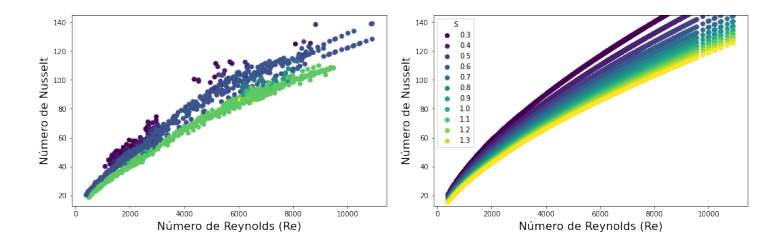
\includegraphics[width=0.9\textwidth]{Captura de pantalla 2025-10-20 184649.png}
  \caption{Número de nusselt en función de número de Reynolds en \cite{DeLaSotta2023}} % El título que va debajo
  \label{fig:mi_grafico} % La etiqueta para referenciarla
\end{figure}